%\title{Title page with logo}
%----------------------------------------------------------------------------------------
%	PACKAGES AND OTHER DOCUMENT CONFIGURATIONS
%----------------------------------------------------------------------------------------

\documentclass[12pt]{article}

%Font and Language
\usepackage[english]{babel}
\usepackage[utf8]{inputenc}
\usepackage{amsmath,amsfonts,amssymb}
\RequirePackage{lmodern}
\RequirePackage[scaled]{helvet}
\RequirePackage[T1]{fontenc}
\RequirePackage{lettrine} 

%Grpahics
\usepackage{graphicx}
\usepackage[colorinlistoftodos]{todonotes}

% Bibliography
\RequirePackage[babel]{csquotes}
\RequirePackage[backend=biber, style=numeric-comp,maxnames=99,maxalphanames=5]{biblatex}
\usepackage[algo2e]{algorithm2e} 


\addbibresource{mybib.bib}

\begin{document}

\begin{titlepage}

\newcommand{\HRule}{\rule{\linewidth}{0.5mm}} % Defines a new command for the horizontal lines, change thickness here

\center % Center everything on the page
 
%----------------------------------------------------------------------------------------
%	HEADING SECTIONS
%----------------------------------------------------------------------------------------

\textsc{\LARGE University of Applied Sciences Ulm}\\[1.5cm] % Name of your university/college
\textsc{\Large Robocup Logistics League}\\[0.5cm] % Major heading such as course name
\textsc{\large Smartbots Ulm}\\[0.5cm] % Minor heading such as course title

%----------------------------------------------------------------------------------------
%	TITLE SECTION
%----------------------------------------------------------------------------------------

\HRule \\[0.4cm]
{ \huge \bfseries Technical Report}\\[0.4cm] % Title of your document
\HRule \\[1.5cm]
 
%----------------------------------------------------------------------------------------
%	AUTHOR SECTION
%----------------------------------------------------------------------------------------

\begin{minipage}{0.4\textwidth}
\begin{flushleft} \large
\emph{Author:}\\
Antoine \textsc{Bretecher} \\% Your name
Peter \textsc{Franzreb} \\% Your name
Matthias \textsc{Goetz} \\% Your name
Florian \textsc{Unger} \\% Your name
\end{flushleft}
\end{minipage}
~
\begin{minipage}{0.4\textwidth}
\begin{flushright} \large
\emph{Supervisor:} \\
Dr. Christian \textsc{Schlegel} % Supervisor's Name
\end{flushright}
\end{minipage}\\[2cm]

% If you don't want a supervisor, uncomment the two lines below and remove the section above
%\Large \emph{Author:}\\
%John \textsc{Smith}\\[3cm] % Your name

%----------------------------------------------------------------------------------------
%	DATE SECTION
%----------------------------------------------------------------------------------------

{\large \today}\\[2cm] % Date, change the \today to a set date if you want to be precise

%----------------------------------------------------------------------------------------
%	LOGO SECTION
%----------------------------------------------------------------------------------------


\includegraphics{pic/logo.png}\\[1cm] % Include a department/university logo - this will require the graphicx package
 
%----------------------------------------------------------------------------------------

\vfill % Fill the rest of the page with whitespace

\end{titlepage}

\tableofcontents

\listoffigures

\listoftables

%\listofalgorithms

\newpage


\begin{abstract}
	THIS IS THE ABSTRACT
\end{abstract}

\section{Introduction}
	THIS IS THE INTRODUCTION

\section{Some \LaTeX{} Examples}
\label{sec:examples}

\subsection{Sections}

Use section and subsection commands to organize your document. \LaTeX{} handles all the formatting and numbering automatically. Use ref and label commands for cross-references.

\subsection{Comments}

Comments can be added to the margins of the document using the \todo{Here's a comment in the margin!} todo command, as shown in the example on the right. You can also add inline comments too:

\todo[inline, color=green!40]{This is an inline comment.}

\subsection{Tables and Figures}

Use the table and tabular commands for basic tables --- see Table~\ref{tab:widgets}, for example. You can upload a figure (JPEG, PNG or PDF) using the files menu. To include it in your document, use the includegraphics command as in the code for Figure~\ref{fig:frog} below.

% Commands to include a figure:

\begin{figure}%[tbhp]
\centering
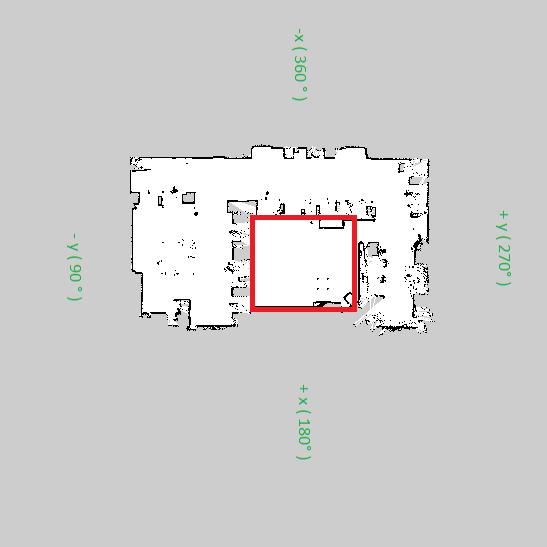
\includegraphics[width=.9\linewidth]{pic/localization-map.png}
\caption{Example picture}
\label{fig:frog}
\end{figure}

\begin{table}
\centering
\begin{tabular}{l|r}
Item & Quantity \\\hline
Widgets & 42 \\
Gadgets & 13
\end{tabular}
\caption{\label{tab:widgets}An example table.}
\end{table}

\subsection{Mathematics}

\LaTeX{} is great at typesetting mathematics. Let $X_1, X_2, \ldots, X_n$ be a sequence of independent and identically distributed random variables with $\text{E}[X_i] = \mu$ and $\text{Var}[X_i] = \sigma^2 < \infty$, and let
$$S_n = \frac{X_1 + X_2 + \cdots + X_n}{n}
      = \frac{1}{n}\sum_{i}^{n} X_i$$
denote their mean. Then as $n$ approaches infinity, the random variables $\sqrt{n}(S_n - \mu)$ converge in distribution to a normal $\mathcal{N}(0, \sigma^2)$.

\subsection{Lists}

You can make lists with automatic numbering \dots

\begin{enumerate}
\item Like this,
\item and like this.
\end{enumerate}
\dots or bullet points \dots
\begin{itemize}
\item Like this,
\item and like this.
\end{itemize}

We hope you find write\LaTeX\ useful, and please let us know if you have any feedback using the help menu above. 
TestCite1 \cite{bir} 
TestCite2 \cite{pycl} 
TestCite3 \cite{spata}

\section{Components}

\subsection{Overview}
	This chapter shall give an overview of the current states of the particular components including the SmartAlvarTagDetection, the SmartRobotinoInstructionPlanner, the Refbox and the SmartMPSDocking components. Each chapter gives an insight on how the component works, how the component is modelled, tested and integrated in the masterdeployment
	
\subsection{SmartAlvarTagDetection}
	 \subsubsection{Overview}


This section is about the SmartAlvarTagDetection Component. The component is used to identify the Alvar Tags on the MPS machines, which is required for the exploration phase where the robots have to explore the game field and find MPS machines and identify the MPS based on their Alvar Tag. \\

Each MPS has their own Alvar Tag, one in the front and one in the back of the machine. This is important for the production phase later. On the field there are seven machines for each team. There are four types of MPS Machines, Base station, Cap station, Ring station and Storage station. All together there are 14 machines with 28 Alvar Tags. \\
Bild von Alvar Tag auf einer MPS. \\

The main idea is that the SmartAlvarTagDetection component identifies the tags. To do so, the component uses an algorithm to determine the Alvar Tag. Therefore, the component needs a picture of the Tag which is taken by a webcam mounted on each of the robotinos and operated by the SmartUnicapImageServer. The SmartAlvarTagDetection components is only one out of many components that are operated and instructed by the InstructionPlanner via the Sequencer (LISPServer). \\
Explain how to operate SmartAlvarTagDetection and SmartUnicapImageServer with DeploymentAlvarTagTest

\subsubsection{CommObjects}

This section describes the CommObjects that are used to communicate with the InstructionPlanner and other componentes.

\subsubsection{Previous State}

The team from the previous semester already had an implementation of the SmartAlvarTagDetection. In their version, they only had implemented the algorithm to scan pictures and identify whether there is a tag or not. They could not communicate with other components or the InstructionPlanner. \\

\begin{figure}[h]
\centering
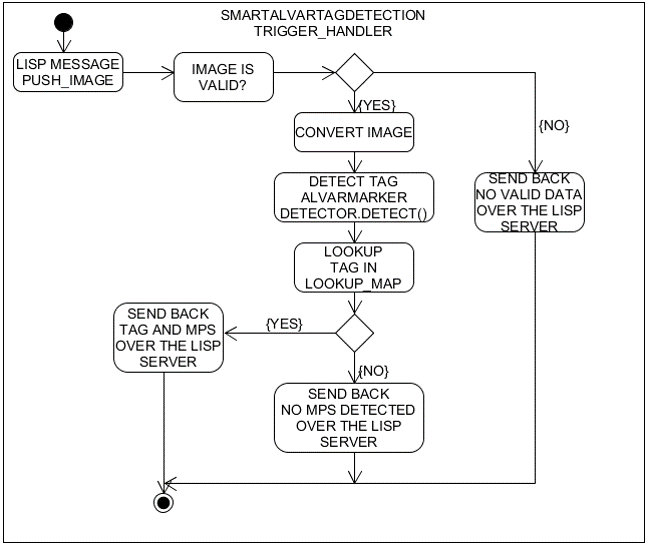
\includegraphics[scale=0.5]{pic/SmartAlvarTagDetectionFlow.png}
\caption{Describes the flow of the SmartAlvarTagDetection Trigger Handler}
\label{fig:smartAlvarFlow}
\end{figure}


At first, the SmartUnicapImageServer is being activated to take a picture and push an image to the SmartAlvarTagDetection. If the SmartUnicapImageServer is done, the LISP Server starts the SmartAlvarTagDetection Trigger Handler. The first thing the Trigger Handler does, is performing a validity check on the picture, to see if the picture can be used or not. If it is not valid, it returns a message saying that the image is not valid. But if it is valid, the image is converted into a greyscale picure, making it easier to recognize the Alvar Tags. Next, the marker detector has to detect an Alvar Tag on the image. It determines the ID by detecting and scanning the tag. In a lookup table this ID is searched and if there is a tag belonging to the ID, then this marker is returned. Markers consist of the type of station, the side and the team color. If the ID cannot be found an error message is returned, otherwise a positive message is returned. \\
Bild von Lookup table \\

The main Problem in this approach was the weak error handling. When for instance no ID could be found on the image and therefore the lookup was not possible, then the entire Robotino crashed. Another problem was that there was no proper communication with the SmartRobotinoInstructionPlanner. When the MPS was detected and found in the lookup table, the positive message was directly sent to the RefBoxServer and not to the SmartRobotinoInstructionPlanner. The communication flow was not transparent. Another problem, not with the implementation but rather with the Alvar and OPENCV libraries, was that it only was possible to deploy the SmartAlvarTagDetection on one computer. Due to difficulties of installing the libraries.



\subsubsection{Current State}

The current version, which was used in the 2017 RoboCup German Open Logistics Leauge in Magdeburg, is able to identify the tags, communicate with the InstructionPlanner via the LISP Server and has some sort of error handling. When the SmartAlvarTagDetection returns the message, that no tag was found, the InstructionPlanner keeps triggering the component five times and if it still sends no tag was found, one can be sure that there really is no tag and it is not a problem with the algorithm or bad picture quality. \\

\begin{figure}[h]
\centering
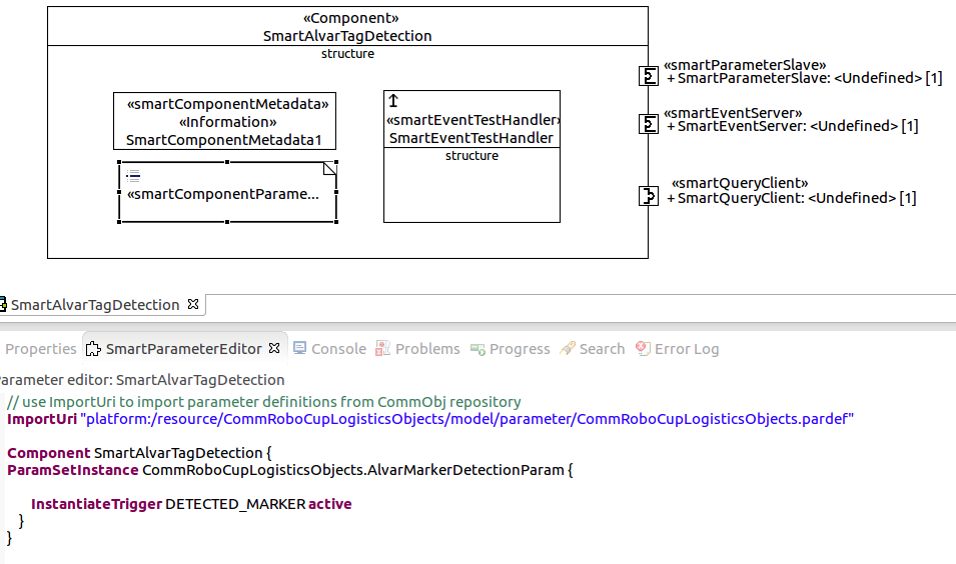
\includegraphics[scale=0.5]{pic/DeploymentAlvarTag.png}
\caption{Shows the model of the SmartAlvarTagDetection component}
\label{fig:smartAlvarFlow}
\end{figure}



The current model consists of a smartEventServer port, a smartQueryClient port and a smartParameterSlave port, but described will be only the first two. The smartEventServer is connected to the LISP Servers' visualMarkerEventClient, which is used to trigger the SmartAlvarTagDetection Trigger Handler.
The other is the SmartQueryClient which is connected to the SmartUnicapImageServers' imageQueryServer to push images that are taken by the webcam to the SmartAlvarTagDetection. The other noticable thing is the smartComponentParameter, which defines the behavior of the SmartAlvarTagDetection component to a Trigger behavior. The smartEventTestHandler is used to check whether an Event fires accordingly. In this case, it tests whether the correct MarkerDetectionState has been set. MarkerDetectionStates are the detected MPS as states. For instance, the tag with ID = 1 has been detected, then the MarkerDetectionState is set to MARKER CYAN CAP STATION 1 FRONT.

	
\subsection{SmartRobotinoInstructionPlanner}
	This is the InstructionPlanner

test for commiting


\subsection{SmartLogisticsRefboxServer}
	
\subsubsection{General}

The Referee Box (Refbox) is an external component build by Aachen University. This component controls, monitors, and evaluates the game during the Robocup. It communicates with robots of both teams and the MPS, attributes the points and manages the different phases of the game. To get more information, it is recommended to read the referee box manual located at \url{http://www.robocuplogistics.org/refbox}. To parametrize the Refbox, the file “config.yaml” should be modify. The most important part to change inside this file is the ip addresses.
 

\subsubsection{Old situation}

There was no permanent Refbox installed in the laboratory. Each team was forced to install on PC in the lab or on his own computer a Refbox with all necessary libraries.


\subsubsection{Current situation}

During this year, a permanent Refbox with all the necessary libraries for the Robocup 2017 version (tneumann/rcll17) have been installed on an independent laptop. Any person that need to test situations with the Refbox can take easily the laptop near his computer or access with XTightVncViewer.  To do this, it is necessary to run the server on the laptop with the command “tightvncserver”. Then it possible to access with the command “xtightvncviewer <<ipAdress>> :1”.  In the current network, the ip address was “172.26.1.112”. The Refbox changes regularly so it is necessary to update each new stable version of the Refbox. All versions can be seen with this link: https://git.fawkesrobotics.org/llsf-refbox.git. A contact with Tim Niemueller, one of the main developer of the Refbox, should be established to know the good version.


\subsubsection{Difficulties}

During the Robocup 2017, some difficulties have been faced. First, it is not possible to choose a zone for a MPS with the Refbox. It results that a successful test is more difficult to do in a smaller area. With this problem, we have use only check if the Refbox can detect the MPS report from robotinos. We were not interested by a correct report. Indeed, there are not MPS in the center of the field with the current generation done by the Refbox. Another problem was to get the last version of the Refbox. Indeed, the current version in the trunk during the Robocup was the Refbox 2016. It was needed to search in a branch to find the correct version of the Refbox. The setting of the network was not easy during the Robocup.


	
\subsection{SmartMPSDockingRobocup}
	This is the MPSDockingDetection

\printbibliography

\end{document}